% TO DO
%
% 1. Images : for title page and inline (get something from creative commons)

\documentclass[a4paper]{module}

\usepackage{lipsum}     % generates filler text, not needed in a real project

\renewcommand*\familydefault{\rmdefault} % select font \sfdefault for sans-serif or \rmdefault for serif

\begin{document}

\title{Dungeon Module X2$\varepsilon$\\
A \LaTeX~Adventure Module Class}

\author{by Michael Davis}

\subtitle{Introductory module for character levels 1--3}

\abstract{This template is provided as a resource for authors of adventure modules for fantasy roleplaying games.
The template requires \LaTeX, a free document preparation system for high-quality typesetting. Unlike a conventional
word processor, the \LaTeX~philosophy is to separate the job of writing content from the job of typesetting it for
publication. The idea is that authors can produce beautifully laid out documents without needing to know anything
about typesetting. It also frees authors from all that fiddly adjusting fonts and resizing images. Another advantage
is that all documents produced using this template will have a similar look and feel, so it's ideal if you want to
publish a series of works.

Using this template as an example, you can write your adventure and turn it into a perfectly-formatted PDF in a few
clicks. You are free to use this for your private texts or for works you distribute for free or commercially (see
details of the license below). Have fun, and unleash your creativity on an unsuspecting world!}

\copyrightblock{This document is formatted using the \LaTeX~module class. Copyright \textcopyright 2016 Michael Davis.

The module class is distributed under the Creative Commons Attribution ShareAlike license version 3.0. In brief, this
grants you the right to \textbf{Share} (copy and redistribute the material in any medium or format) and \textbf{Adapt}
(remix, transform and build upon the material for any purpose, even commercially) the class under the following terms:
\textbf{Attribution} (you must give appropriate credit, provide a link to the license, and indicate if changes were made.
You may do so in any reasonable manner, but not in any way that suggests the licensor endorses you or your use),
\textbf{ShareAlike} (if you remix, transform, or build upon the material, you must distribute your contributions under
the same license as the original) and \textbf{No additional restrictions} (you may not apply legal terms or technological
measures that legally restrict others from doing anything the license permits). See the copyright information at the
end for more details.

Some parts of this class, namely the monster stat blocks, are Copyright \textcopyright 2000--2003 Wizards of the Coast
and are distributed under the Open Gaming License.

If you want to use the OGL stat blocks or other OGL material, the template includes some handy macros for adding the OGL
license to your work. If you are not using any OGL material you can omit those from your document.}

\contactblock{
% supply logo as an argument
Contact me as slithy on DragonsFoot
}

\maketitle

\part{Introduction}

The first thing you need to be aware of is that LaTeX uses a markup language in order to describe document structure and presentation. What LaTeX does is to convert your source text, combined with the markup, into a high quality document. For the purpose of analogy, web pages work in a similar way: the HTML is used to describe the document, but it is your browser that presents it in its full glory - with different colours, fonts, sizes, etc.

\part{Usage}

% \documentclass[a4paper]{dnd_module}
%
% Accepts 'letter' or 'a4paper' options to specify page size. The amount of text on each page is not changed;
% the only difference between the two options is the size of the top margin and left/right margins. This allows
% module writers to easily create two almost identical PDFs for use in USA and Europe/rest of the world.

\section{Fonts}

% Choose \rmdefault to select the serifed font and \sfdefault for a sans-serif font
% If you are using the serifed font, the ITC Souvenir, the font used in the Moldvay Basic rulebook from 1981)

\section{Monster Stat Blocks}

\monster{kobold}{Kobold}{7|$1/2$|60' (20')|weapon|1d4|NM|6|C}
\monster{harpy}{Harpy}{7|3*|20'/50'|2 claws and a weapon + charm|1d4/1d4/1d6|F6|6|C}
\monster[Octopodes]{octopus}{Octopus}{7|3*|20'/50'|8 legs|1d6 each|F6|6|C}
\monster{platypus}{Platypus}{7|3*|20'/50'|bill|1d4|F6|6|C}

First stat block:
\statblock{kobold}{5}{4,4,3,2,1}
Second stat block:
\statblock{kobold}{1}{3}

You must face the \stats[Kobold King!]{kobold}{1}{4}. 
He is with his \stats[10 bodyguards: ]{kobold}{10}{4 each}

\statblock{harpy}{1}{10}
\statblock{harpy}{3}{24 each}

\statblock{octopus}{1}{10}
\statblock{octopus}{3}{24 each}

\statblock{platypus}{1}{10}
\statblock{platypus}{3}{24 each}

\begin{statblockfreestyle}
Jim the Rogue: leather armour, small fruit knife, S7 I12 W5 D17 C12 Ch15. He can backstab with +4 to hit and double damage. AL C
\end{statblockfreestyle}

%%%%% Level One %%%%%

\part{First Dungeon Level}

Some introductory text for the DM.

\subsection{Key to Dungeon Level One}

\subsubsection*{Start}

\boxtext{Some boxed text to read to the players to introduce them to the adventure.}

\subsubsection{The Gatehouse}

\boxtext{It looks dangerous.}

Some monsters are here.

\subsubsection{The Secret Entrance}

\boxtext{You see some bushes.}

If the players investigate, they will find a hidden trapdoor under the bushes. Under the trapdoor is a tunnel leading under the wall.

\subsubsection{The big bad end guy}

\begin{figure}[h]
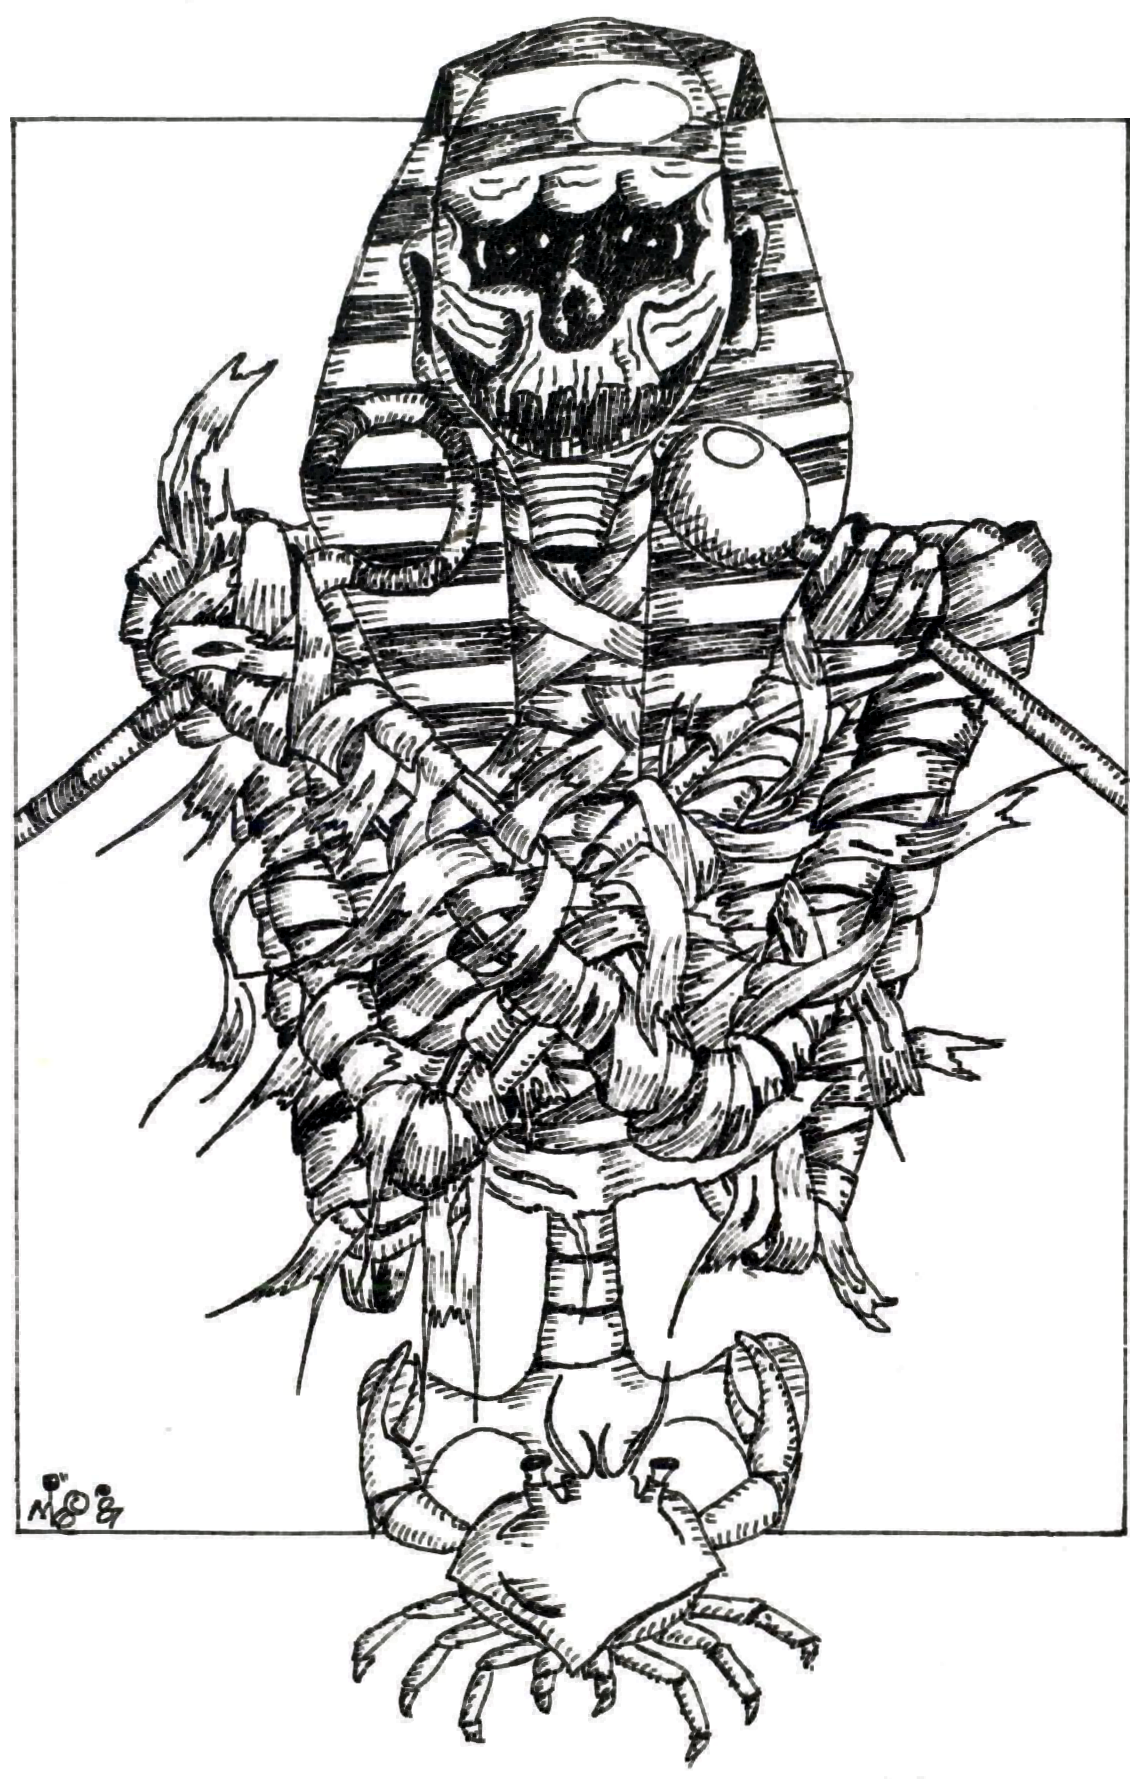
\includegraphics[width=\columnwidth]{module_art_interior.png}
\center{Tomb It May Concern.\\
Image Copyright \textcopyright 1987, 2016 Michael Davis.}
\end{figure}

%%%%% Level Two %%%%%

\begin{minipage1col}[b]
\part{Second Dungeon Level}

The \texttt{\textbackslash onecolumn} command can be used to switch into single column mode. \texttt{\textbackslash twocolumn} switches back to two-column mode. However,
these commands do not allow mixing one- and two-column text on the same page. If you would like to have just part of a page in one-column mode, use the custom
environment \texttt{minipage1col}.

\subsection{Wandering Monsters}

\lipsum
\end{minipage1col}

\lipsum

\section{Open Game Content}

The template includes macros to make it easy to distribute your work under the Open Game License from Wizards of the Coast.

\begin{ogl}
\item Here include the exact text of the COPYRIGHT NOTICE of any other OGL text you are copying, modifying or distributing.
\item Add the title, copyright date and copyright holder's name(s) of any OGL content you distribute. Example:
\item System Reference Document, Copyright 2000--2003, Wizards of the Coast, Inc., by Jonathan Tweet, Monte Cook, Skip Williams, Rich Baker, Andy Collins,
David Noonan, Rich Redman, Bruce R. Cordell, John D. Rateliff, Thomas Reid, James Wyatt, based on original material by E. Gary Gygax and Dave Arneson.
\end{ogl}

\begin{productidentity}
\item The \LaTeX~module class and example template, which comprises all typesetting elements and all text which is not explitly Open Game Content, is Product Identity.
\modulecopyright

\item All artwork in this template is Product Identity. Copyright belongs to the artists, all rights reserved.
\end{productidentity}

\begin{opengamecontent}
\item The monster statistics from the SRD are Open Game Content.
\end{opengamecontent}

\end{document}
